\section{Comparing Attributes}
To be able see if any of the attributes have had a big effect on whether the different subjects got CHD, we plotted some of the attributes against each other.

\subsection{Tobacco vs. Alcohol}

Some of the attributes we thought would be interesting to compare to each other, were amongst other tobacco and alcohol, since these are often considered bad for your health. In figure \ref{AlcoTobac} we can see those two attributes plotted against each other. It does look like that tobacco has a bigger influence on CHD than alcohol, but we cannot tell that much more about these two from this figure since the spread of negative and positive seems very similar. However it seems like people located in the extremes, meaning smoking and drinking a lot, are more exposed to the disease.

\begin{figure}[H]
\centering
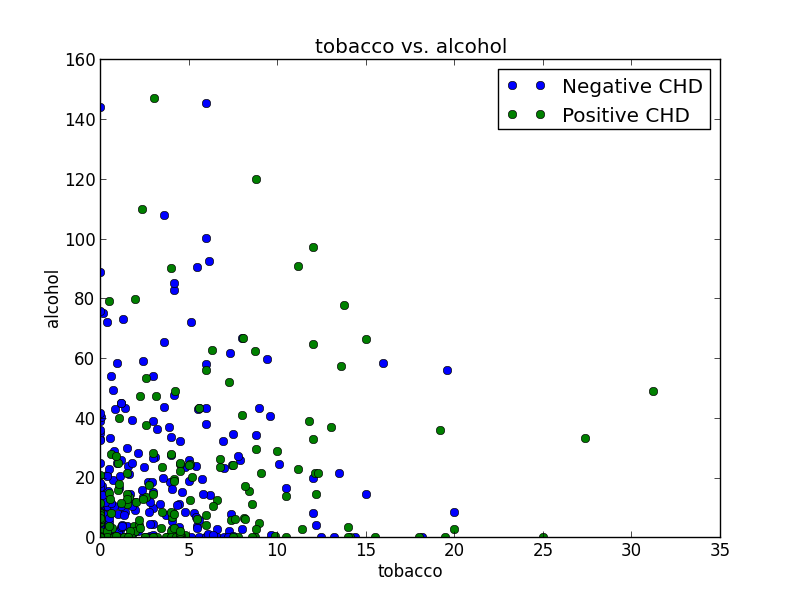
\includegraphics[width=7cm, keepaspectratio=true]{pictures/tobaccoAlcohol.png}
\vspace{-0.4cm}
\caption{\footnotesize Tobacco vs. Alcohol}
\label{AlcoTobac}
\end{figure}

\subsection{Obesity vs. Adiposity}

Alcohol and tobacco was not the only attribute we thought would be interesting to look at, we also thought of what the more obese subject would look like. In figure \ref{ObeAsi} we see the adiposity and obesity put up against each other. First of all, we see that the two attributes depends a lot on each other, which we would also expect. The tendency of the graph is that the higher adiposity, the higher obesity. However two subjects, in the top-left corner and the bottom-right corner, stand out from the rest. These two are different than the others, since they lie far from mass of subject that gathers in a bit bend line. This could be the result of wrong data. But these are considered outliers in this comparison.

When you look at figure \ref{ObeAsi} you see that the higher the values get the more subjects got CHD. This could mean that the higher values a subject got in adiposity and obesity, the bigger chance is there for the subject to get CHD.

\begin{figure}[H]
\centering
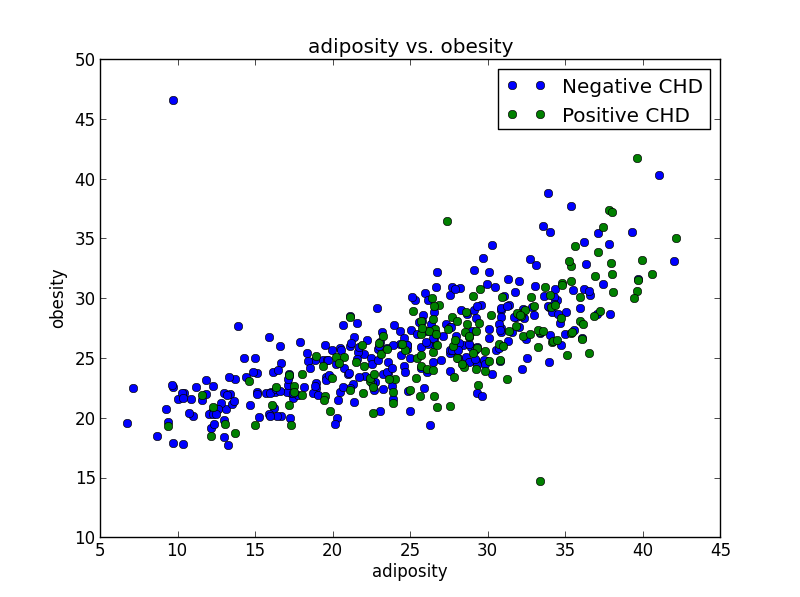
\includegraphics[width=7cm, keepaspectratio=true]{pictures/adiposityObesity.png}
\vspace{-0.4cm}
\caption{\footnotesize Adiposity vs. Obesity}
\label{ObeAsi}
\end{figure}

\subsection{Type-a vs. Alcohol}

In figure \ref{typeAlco} we try to see if more aggressive subjects have a higher chance on getting CHD, and if alcohol would make difference in how aggressive subjects would be. What we can see in the figure is at first that alcohol does not seem to have a big influence on how aggressive the different subjects are. But it does seem like very aggressive people have a higher chance of being positive for CHD. In general it seems like there is a similar spread in both positive and negative tested subjects.

\begin{figure}[H]
\centering
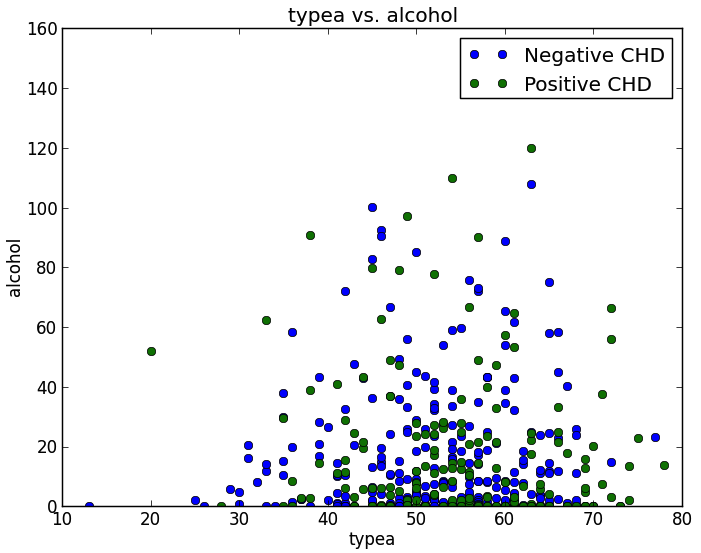
\includegraphics[width=7cm, keepaspectratio=true]{pictures/typeaalcohol.png}
\vspace{-0.4cm}
\caption{\footnotesize Type-a vs. Alcohol}
\label{typeAlco}
\end{figure}